\documentclass[12pt, twoside]{book}
%\documentclass[12pt, oneside]{book}  % jednostranna tlac

%spravne nastavenie okrajov
\usepackage[a4paper,top=2.5cm,bottom=2.5cm,left=3.5cm,right=2cm]{geometry}
%zapnutie fontov pre UTF8 kodovanie
\usepackage[utf8]{inputenc}
\usepackage[T1]{fontenc}

%zapnutie slovenskeho delenia slov
%a automatickych nadpisov ako Obsah, Obrázok a pod. v slovencine
%\usepackage[slovak]{babel} % vypnite pre prace v anglictine!

%nastavenie riadkovania podla smernice
\linespread{1.25} % hodnota 1.25 by mala zodpovedat 1.5 riadkovaniu

% balicek na vkladanie zdrojoveho kodu
\usepackage{listings}
% ukazky kodu su cislovane ako Listing 1,2,...
% tu je Listing zmenene na Algoritmus 1,2,...
\renewcommand{\lstlistingname}{Algorithm}
% nastavenia balicka listings
% mozete pridat aj language=...
% na nastavenie najcastejsie pouzivaneho prog. jazyka
% takisto sa da zapnut cislovanie riadkov
\lstset{frame=lines}
% Style for pseudocode listings
\lstdefinestyle{pseudocode}{
    frame=lines,
    basicstyle=\ttfamily\small,
    keywordstyle=\bfseries,
    morekeywords={Input,Output,Repeat,Until,Return,if,then,else,while,do,for,swap},
    mathescape=true,
    escapeinside={(*}{*)},
    columns=fullflexible,
    keepspaces=true,
    xleftmargin=2em,
    aboveskip=1.5em,
    belowskip=1.5em,
    numbers=left,              % line numbers on the left
    numberstyle=\tiny\color{gray}, % line number style
    numbersep=10pt,             % gap between numbers and code
    stepnumber=1,
}

% balicek na vkladanie obrazkov
\usepackage{graphicx}
\usepackage{subcaption}
% balicek na vkladanie celych pdf dokumentov, tu zadanie
\usepackage{pdfpages}
% balicek na matematicke vzorce
\usepackage{amsmath}
% balicek na spravne formatovanie URL
\usepackage{url}
% balicek na hyperlinky v ramci dokumentu
% zrusime farebne ramiky okolo liniek aby pdf
% vyzeralo rovnako ako tlacena verzia
\usepackage[hidelinks,breaklinks]{hyperref}
% triedenie citacii
\usepackage[sort]{cite}

\usepackage{amssymb}

% nice line
\usepackage{booktabs}

\usepackage{multirow}

\usepackage{float}


% -------------------
% --- Definicia zakladnych pojmov
% --- Vyplnte podla vasho zadania, rok ma byt rok odovzdania
% -------------------
\def\mfrok{2026}
\def\mfnazov{Permuting Matrix Columns for Improved Block-Sparse Pruning}
\def\mftyp{Master Thesis}
\def\mfautor{Bc. Jitka Muravská}
\def\mfskolitel{Mgr. Vladimír Boža, PhD.}

%ak mate konzultanta, odkomentujte aj jeho meno na titulnom liste
% \def\mfkonzultant{tit. Meno Priezvisko, tit. }  

\def\mfmiesto{Bratislava, \mfrok}

% študenti BIN a DAV odkomentujú príslušnú dvojicu riadkov
\def\mfodbor{Computer Science}
\def\program{Computer Science }
% pre BIN:
%\def\mfodbor{Computer Science and Biology} 
%\def\program{ Bioinformatics }
% pre DAV:
%\def\mfodbor{Computer Science and Mathematics} 
%\def\program{ Data Science }

% Ak je školiteľ z FMFI, uvádzate katedru školiteľa, zrejme by mala byť aj na zadaní z AIS2
% Ak máte externého školiteľa, uvádzajte Katedru informatiky 
\def\mfpracovisko{ Department of Applied Informatics }

\begin{document}     
\frontmatter
\pagestyle{empty}

% -------------------
% --- Obalka ------
% -------------------

\begin{center}
  \sc\large
  Comenius University in Bratislava\\
  Faculty of Mathematics, Physics and Informatics

\vfill

{\LARGE\mfnazov}\\
\mftyp
\end{center}

\vfill

{\sc\large 
\noindent \mfrok\\
\mfautor
}

\cleardoublepage
% --- koniec obalky ----

% -------------------
% --- Titulný list
% -------------------

\noindent

\begin{center}
\sc  
\large
  Comenius University in Bratislava\\
  Faculty of Mathematics, Physics and Informatics

\vfill

{\LARGE\mfnazov}\\
\mftyp
\end{center}

\vfill

\noindent
\begin{tabular}{ll}
Study Programme: & \program \\
Field of Study: & \mfodbor \\
Department: & \mfpracovisko \\
Supervisor: & \mfskolitel \\
% Consultant: & \mfkonzultant \\
\end{tabular}

\vfill


\noindent \mfmiesto\\
\mfautor

\cleardoublepage
% --- Koniec titulnej strany


% -------------------
% --- Zadanie z AIS
% -------------------
% v tlačenej verzii s podpismi zainteresovaných osôb.
% v elektronickej verzii sa zverejňuje zadanie bez podpisov
% v pracach v anglictine anglicke aj slovenske zadanie

\newpage
\setcounter{page}{3}
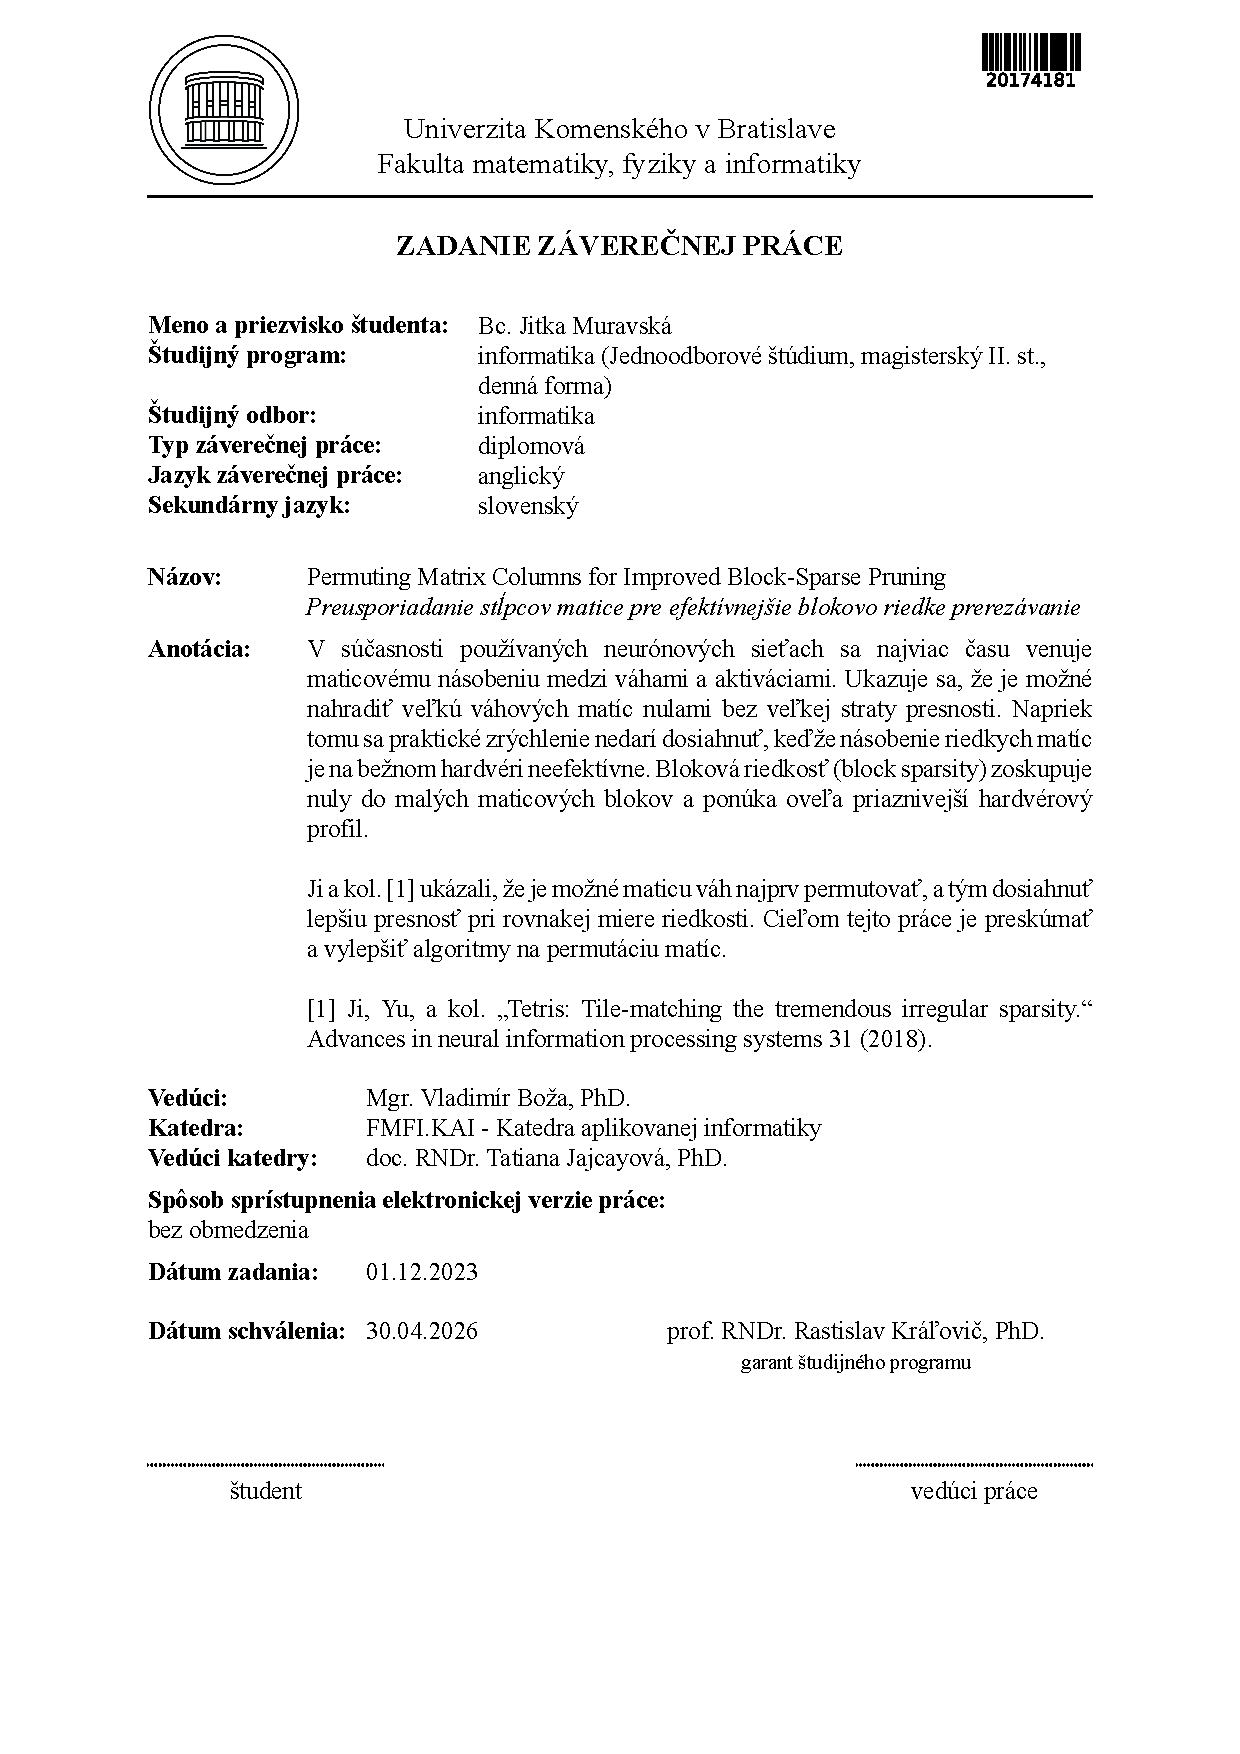
\includepdf{images/zadanie.pdf}

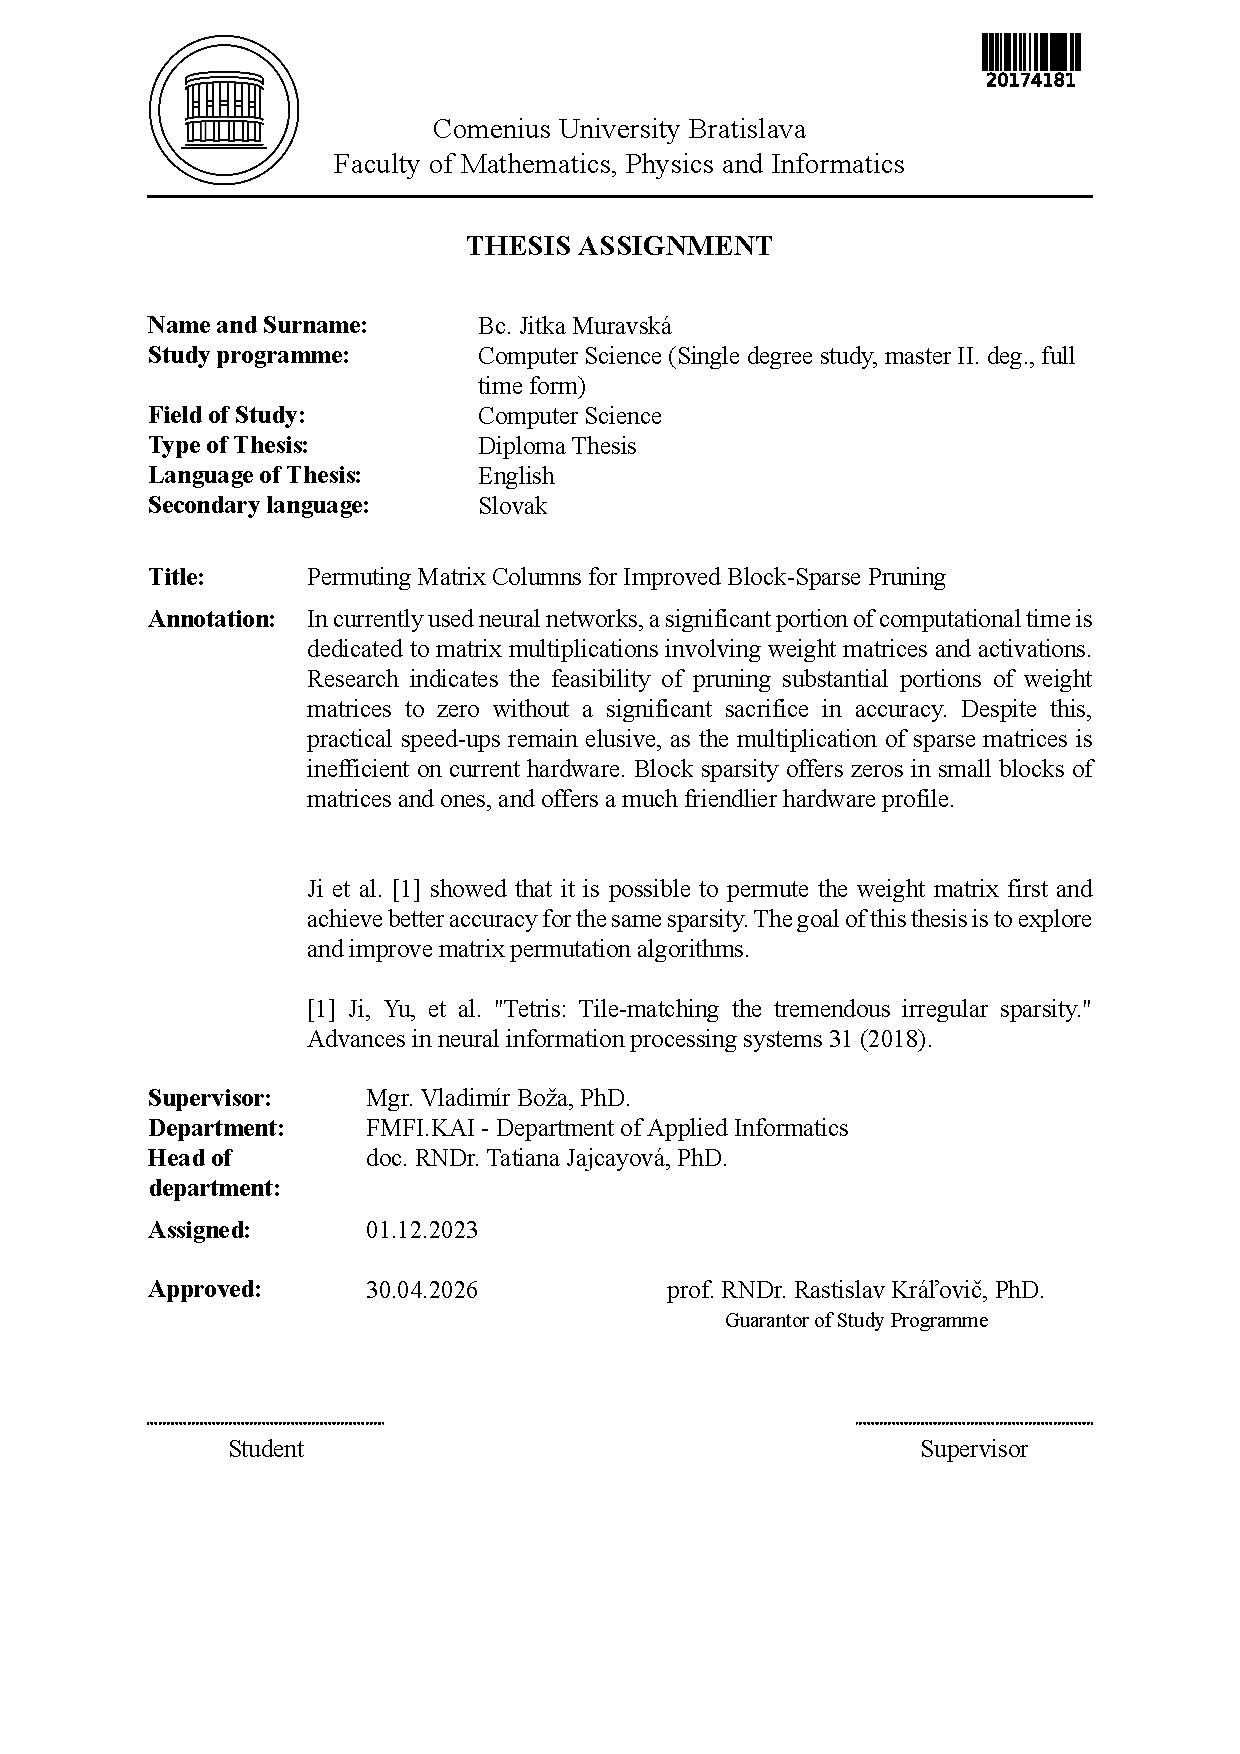
\includepdf{images/zadanie-en.pdf}

% --- Koniec zadania


% -------------------
%   Poďakovanie - nepovinné
% -------------------
\newpage
\pagestyle{plain}
~

\vfill
{\bf Declaration of Honour:} I declare that I have written the entire diploma thesis "Permuting Matrix Columns for Improved Block-Sparse Pruning", including all its appendices and figures, independently, using only the literature listed in the attached bibliography and with the assistance of artificial intelligence tools. I declare that the use of AI tools was in accordance with applicable legal regulations, academic rights and freedoms, ethical and moral principles, and that I have maintained academic integrity throughout the process. The following AI tools were used in the preparation of this thesis: Claude — for rewording text, assistance with LaTeX, help with implementing code for generating figures, and code formatting. The author is responsible for the correctness of the final form of the text.

{\bf Acknowledgments:} I would like to thank my supervisor for his guidance and cheering me on when I thought nothing was working. For the emotional support, the gratitude goes also to my family and friends, especially to my boyfriend for his patience, understanding, and never-ending support during the stressful times of writing this thesis.
% --- Koniec poďakovania

% -------------------
%   Abstrakt - Slovensky
% -------------------
\newpage 
\section*{Abstrakt}

Moderné transformerové modely, od veľkých jazykových modelov po vizuálne transformery (angl. Vision Transformer), dosahujú pôsobivé výsledky na úlohách, no pri inferencii vyžadujú značné výpočtové a pamäťové zdroje. Orezávanie znižuje tieto náklady tým, že časť váh nastaví na nulu, ideálne s malou alebo žiadnou stratou kvality modelu. Blokové orezávanie robí výsledný vzor riedkosti priaznivejším pre hardvér, no za cenu: zoskupovanie váh do blokov pred orezávaním môže uväzniť dôležité váhy v inak málo hodnotných blokoch. Algoritmus TETRIS \cite{tetris} tento problém rieši permutovaním prvkov podľa dimenzií matice váh pred orezávaním, pričom na nájdenie dobrých permutácií používa nenásytné lokálne vyhľadávanie. V tejto práci predstavujeme Global Assignment TETRIS (GA-TETRIS), variant, ktorý nahrádza lokálne vyhľadávanie presným riešením úlohy minimálneho váženého bipartitného párovania v každej iterácii, doplnené o injektovanie šumu a vylepšovanie pomocou náhodných výmen na únik z lokálnych optím. GA-TETRIS porovnávame s pôvodným algoritmom TETRIS, troma jednoduchšími heuristikami (Sort-by-Norm, Random-Swaps a Random-Swaps so zoradenou inicializáciou) a so základným riešením Block-Wanda bez permutácie na dvoch Vision Transformeroch (0,9M a 13,4M parametrov) a modeli SmolLM2-360M. Pri cieli orezávania na úrovni jednotlivých vrstiev dosahuje GA-TETRIS najvyššie zlepšenie skóre pri širokých blokoch naprieč všetkými troma modelmi. Pri vyhodnotení celého modelu výkon prudko klesá s rastúcou šírkou bloku pri každom modeli; iba Väčší ViT pri bloku $1 \times 2$ si zachováva podstatnú presnosť. V tomto jedinom režime je GA-TETRIS najlepším algoritmom o 1,85 percentuálneho bodu pred druhým najlepším. Na modeli SmolLM2 pri rovnakej šírke bloku však jednoduchá heuristika Sort-by-Norm produkuje najnižšiu perplexitu — hoci stále približne sedemnásobne horšiu ako neorezaný model — čo naznačuje, že najlepší algoritmus závisí od šírky bloku aj od modelu.

\paragraph*{Kľúčové slová:} blokové orezávanie, lineárne priradenie, TETRIS, permutácia
% --- Koniec Abstrakt - Slovensky


% -------------------
% --- Abstrakt - Anglicky 
% -------------------
\newpage 
\section*{Abstract}

Modern transformer models, from large language models to vision transformers, achieve impressive task performance but require substantial compute and memory at inference. Pruning reduces this cost by zeroing out a fraction of its weights, ideally at little or no loss in task quality. Block pruning makes the resulting sparsity pattern hardware-friendly, but at a cost: grouping weights into blocks before pruning can trap important weights inside otherwise-low-value blocks. The TETRIS algorithm of \cite{tetris} addresses this by permuting the elements along the dimensions of the weight matrix before pruning, using a greedy local search to find good permutations. We propose Global Assignment TETRIS (GA-TETRIS), a variant that replaces the local search with an exact solution to a minimum-weight perfect matching in a bipartite graph problem at each iteration, augmented with noise injection and random-swap refinement to escape local optima. We evaluate GA-TETRIS against the Original TETRIS, three simpler heuristics (Sort-by-Norm, Random-Swaps, and Random-Swaps with sorted initialization), and the no-permutation Block-Wanda baseline on two Vision Transformers (0.9M and 13.4M parameters) and SmolLM2-360M. On the per-layer pruning objective, GA-TETRIS achieves the highest score improvement at wide block widths across all three models. On whole-model evaluation, performance collapses rapidly with growing block width on every model; only the Larger ViT at block $1 \times 2$ preserves substantial accuracy. In that single regime, GA-TETRIS is the best algorithm by 1.85 percentage points over the next best. On SmolLM2 at the same block width, however, the simple Sort-by-Norm heuristic produces the lowest perplexity — though still roughly seven times worse than the unpruned baseline — suggesting that the best algorithm depends on both block width and model.


\paragraph*{Keywords:} block pruning, linear sum assignment, TETRIS, permutation

% --- Koniec Abstrakt - Anglicky

% -------------------
% --- Predhovor - v informatike sa zvacsa nepouziva
% -------------------
%\newpage 
%
%
%\chapter*{Preface} %
%
%Predhovor je všeobecná informácia o práci, obsahuje hlavnú charakteristiku práce 
%a okolnosti jej vzniku. Autor zdôvodní výber témy, stručne informuje o cieľoch 
%a význame práce, spomenie domáci a zahraničný kontext, komu je práca určená, 
%použité metódy, stav poznania; autor stručne charakterizuje svoj prístup a svoje
%hľadisko. 
%
% --- Koniec Predhovor


% -------------------
% --- Obsah
% -------------------

\cleardoublepage 

\tableofcontents

% ---  Koniec Obsahu

% -------------------
% --- Zoznamy tabuliek, obrázkov - nepovinne
% -------------------

\newpage 

% \listoffigures
% \listoftables

% ---  Koniec Zoznamov

\mainmatter
\pagestyle{headings}

\input intro.tex 

\input chapter1.tex
\input chapter2.tex
\input chapter3.tex

\input conclusion.tex



%\input zaver.tex

% -------------------
% --- Bibliografia
% -------------------


\newpage	

\backmatter

\thispagestyle{empty}
\clearpage

\bibliographystyle{plain}
\bibliography{literatura} 

%Prípadne môžete napísať literatúru priamo tu
%\begin{thebibliography}{5}
 
%\bibitem{br1} MOLINA H. G. - ULLMAN J. D. - WIDOM J., 2002, Database Systems, Upper Saddle River : Prentice-Hall, 2002, 1119 s., Pearson International edition, 0-13-098043-9

%\bibitem{br2} MOLINA H. G. - ULLMAN J. D. - WIDOM J., 2000 , Databasse System implementation, New Jersey : Prentice-Hall, 2000, 653s., ???

%\bibitem{br3} ULLMAN J. D. - WIDOM J., 1997, A First Course in Database Systems, New Jersey : Prentice-Hall, 1997, 470s., 

%\bibitem{br4} PREFUSE, 2007, The Prefuse visualization toolkit,  [online] Dostupné na internete: <http://prefuse.org/>

%\bibitem{br5} PREFUSE Forum, Sourceforge - Prefuse Forum,  [online] Dostupné na internete: <http://sourceforge.net/projects/prefuse/>

%\end{thebibliography}

%---koniec Referencii

% -------------------
%--- Prilohy---
% -------------------

%Nepovinná časť prílohy obsahuje materiály, ktoré neboli zaradené priamo  do textu. Každá príloha sa začína na novej strane.
%Zoznam príloh je súčasťou obsahu.
%
\input appendixA.tex

%\input appendixB.tex

\end{document}






